% !TEX root = mythesis.tex

%==============================================================================
\chapter{Theoretical Background}
\label{sec:theoretical_background}
%==============================================================================
\section{Clusters and groups of galaxies}\label{sec:clusters}
Throughout the Universe, galaxies are not distributed homogeneously but are instead aggregated into large cosmic structures known as galaxy groups or galaxy clusters, which are the largest relaxed structures in the Universe. Galaxy clusters typically have masses exceeding \(M \gtrsim 3 \times 10^{14} M_{\odot}\), whereas galaxy groups have masses around \(M \sim 3 \times 10^{13} M_{\odot}\) (\cite{Schneider_2006}). Advancements in X-ray astronomy have demonstrated that these structures are significant sources of X-ray radiation (\cite{Cavaliere_1971}). This emission is well understood to originate from a hot intergalactic gas known as the intracluster medium (ICM)\footnote{The intercluster medium is also called the intragroup medium (IGM) in the case of galaxy groups. In the context of this thesis, the terms ICM and IGM will be used interchangeably, as a distinction between them is not necessary.}, which is characterized by temperatures in the range of \SIrange{e7}{e8}{\kelvin} and constitutes the primary baryonic component of galaxy clusters and groups (\cite{Schneider_2006}).
%
\subsection{The Intracluster Medium}
Within the deep gravitational wells of galaxy clusters and groups, the temperature becomes sufficiently high to fully ionize lighter elements and partially ionize heavier elements, resulting in the formation of a plasma. This hot, diffuse, and optically thin plasma, known as the intracluster medium (ICM), emits a significant amount of X-ray radiation. X-ray observations of the ICM have enabled a wide variety of cosmological studies, including advances in understanding the large-scale structure formation in the Universe (\cite{KravtsovBorgani2012}).
%
\subsection{Emission Processes within the ICM}\label{subsec:emission}
A key principle of electrodynamics is that accelerated charges radiate energy. This radiation is referred to as bremsstrahlung or \enquote{free-free} when a unbound charged particle, typically an electron, is accelerated by the electric field of other charges, usually ions. In the ICM, this process predominates at temperatures above \(k_B T_\text{e} \gtrsim \SI{2}{\kilo\electronvolt}\), where the total emissivity \(\epsilon_{\text{ff}}\) at solar metallicity scales approximately as \(\epsilon_{\text{ff}} \propto T_\text{e}^{0.5} n_\text{e}\), 
with \(n_\text{e}\) and \(T_\text{e}\) as the electron number density and temperature, respectively. At lower temperatures (\(k_B T \lesssim \SI{2}{\kilo\electronvolt}\)), line emission becomes significant, with the emissivity being roughly described by \(\epsilon \propto T_\text{e}^{-0.6} n_\text{e}\).
Thus, for the low energy band \SIrange{0.1}{2.4}{\kilo\electronvolt}, one roughly finds that \(\epsilon \propto n_\text{e}^2.\) (\cite{Reiprich2019}).
%
\subsection{The beta model of the ICM}\label{sec:beta_model}
In the mid-1970s, \cite{Cavaliere_1976} laid the groundwork for the current understanding of the ICM. The X-ray morphology of clusters and groups is typically described by the beta model. This model assumes gas and galaxies share the same gravitational potential. Given a constant temperature \(T\) and velocity dispersion \(\sigma_r\), the radial distributions of the gas \(n_{\text{gas}}\) and galaxies \(\rho_{\text{gal}}\) obey
\begin{align*}
    \frac{n_\text{gas}(r)}{n_{\text{gas}}(0)} = \left[\frac{\rho_{\text{gal}}(r)}{\rho_{\text{gal}(0)}}\right]^{\beta}; \quad \beta = \frac{\mu m_p \sigma_r^2}{k_BT}
\end{align*}
where \(\mu\) is the mean molecular mass, \(m_p\) is the proton mass and \(k_B\) is the Boltzmann constant. Using the King approximation, which d \({\textstyle \rho_{\text{gal}}(r) = \rho_{\text{gal}}(0)[1 + (r/r_c)^2]^{-3/2}}\) (\cite{King1962}) where \(r_c\) is the core radius and \(\epsilon \propto n_e^2\), the X-ray surface brightness \(S_X\), obtained by integrating over the emissivity, follows the profile 
\begin{align*}
    S_X(r) = S_X(0)\left[1 + \left(\frac{r}{r_c}\right)^2\right]^{-3\beta + 1/2}.
\end{align*}
The beta model is widely used to describe cluster and group emissions, despite the assumptions listed above often being unmet. Excess core emission, for example, is typically addressed by adding a second beta model component: \(S_X^{\text{tot}} = S_{X,1} + S_{X,2}\) (\cite{Reiprich2019}).
%
\subsection{The galaxy group NGC1550}\label{sec:ngc1550}
The galaxy group NGC1550 is located at a right ascension of \(\SI{64.9066}{\degree}\) and a declination of \(\SI{2.4151}{\degree}\), with a redshift of \(z = 0.0123\) (\cite{Reiprich_2002}). Although the lenticular galaxy NGC 1550 has long been observable in the optical, it was first associated with the extended X-ray source RX J0419+0225 through the ROSAT All-Sky Survey (\cite{Bohringer_2000}). The presence of this extensive X-ray halo, along with its considerable mass (\(\sim 2 \times 10^{13} M_{\odot}\)), led to its classification as a galaxy group (\cite{Kawaharada_2003}).

Recent studies indicate that NGC1550 does not meet the formal criteria for a fossil group (\cite{Sun_2003}; cf. \cite{Jones2003} for the criteria), but it shares several features with such groups. One notable characteristic is its high X-ray bolometric luminosity (\(\gtrsim \SI{4.8e41}{\erg}\)), which predominantly originates from a central, dominant, early-type galaxy. Fossil groups are thought to be formed when member galaxies in a regular galaxy group merge into a central dominant galaxy, and evidence for this process has been found in the metal distribution of NGC1550 (\cite{Kawaharada_2009, Sato_2010}). Additionally, a recent study has identified signs of AGN (active galactic nucleus) feedback and sloshing, suggesting a minor merger occurred around 33 million years ago (\cite{Kolokythas_2020}). While the group appears to be relaxed overall, a slight east-west elongation in the central region has been noted by multiple authors (\cite{Kolokythas_2020, Sun_2003}).
%
\section{eROSITA}
The \textit{extended ROentgen Survey with an Imaging Telescope Array} (eROSITA) is a highly sensitive, wide-field X-ray telescope designed to capture deep images across large areas of the sky. Mounted on the Spektrum-Roentgen-Gamma (SRG) observatory in a halo orbit around the second Lagrange Point (L2), eROSITA operates within the 0.2 to 10.0 keV energy range. It is the first instrument to perform an all-sky imaging survey in the hard X-ray band (2.0 to 10.0 keV). In the soft X-ray band (0.5 to 2.0 keV), eROSITA boasts a sensitivity that is approximately 20 times greater than that of its predecessor, the ROSAT All-Sky Survey. eROSITA features seven identical mirror modules, known as Telescope Modules (TMs), with 54 mirror shells in Wolter-I geometry and a 1.6-meter focal length. Five TMs (TM1, TM2, TM3, TM4 and TM6) have aluminum on-chip optical light filters and are collectively referred to as TM8. The remaining two TMs (TM5, TM7), designed for low-energy spectroscopy, lack these filters and are referred to as TM9. Collectively, TM8 and TM9 are referred to as TM0. (\cite{Predehl2021}). In this thesis, data from the first all-sky survey (eRASS:1) will be utilized. The data is provided in the form of event lists, which essentially detail the spatial position of X-ray photon arrivals on the detector, their time of arrival, and their energy. The event lists are made available in \(\SI{3.6}{\degree}\times\SI{3.6}{\degree}\) regions known as skytiles.
\section{Sky background and contamination sources}\label{sec:background}
For a thorough analysis of X-ray photons, it is essential to carefully consider both external background and internal instrumental contamination effects. The following section will provide a brief overview of the most important factors relevant to this analysis.
\paragraph*{Cosmic X-ray Background (CXB):} The cosmic X-ray background (CXB) comprises multiple sources, including diffuse, unabsorbed thermal emissions from the Local Hot Bubble, a plasma cavity surrounding the Sun, and absorbed thermal emissions from the Galactic halo (\cite{galeazzi2006xmm}). Additionally, it includes discrete extragalactic sources, predominantly unresolved AGNs  (\cite{brandt2005deep}). The diffuse component is more prominent in the lower energy band \(\sim\SI{1}{\kilo\electronvolt}\), while the extragalactic sources dominate at higher energies. In this analysis, background emission from the nearby Orion-Eridanus superbubble, which spans roughly \SI{40}{\degree} on the sky, shall also be present, as it emits in the soft X-ray regime (\cite{Krause_2014}). Figure \ref{fig:orion_superbubble}, taken from \cite{Krause_2014}, shows an X-ray map of the Orion-Eridanus superbubble in the \SIrange{0.5}{2.0}{\kilo\electronvolt} band, illustrating its overlap with the galaxy group NGC1550.
\begin{figure}[htbp]
    \centering
    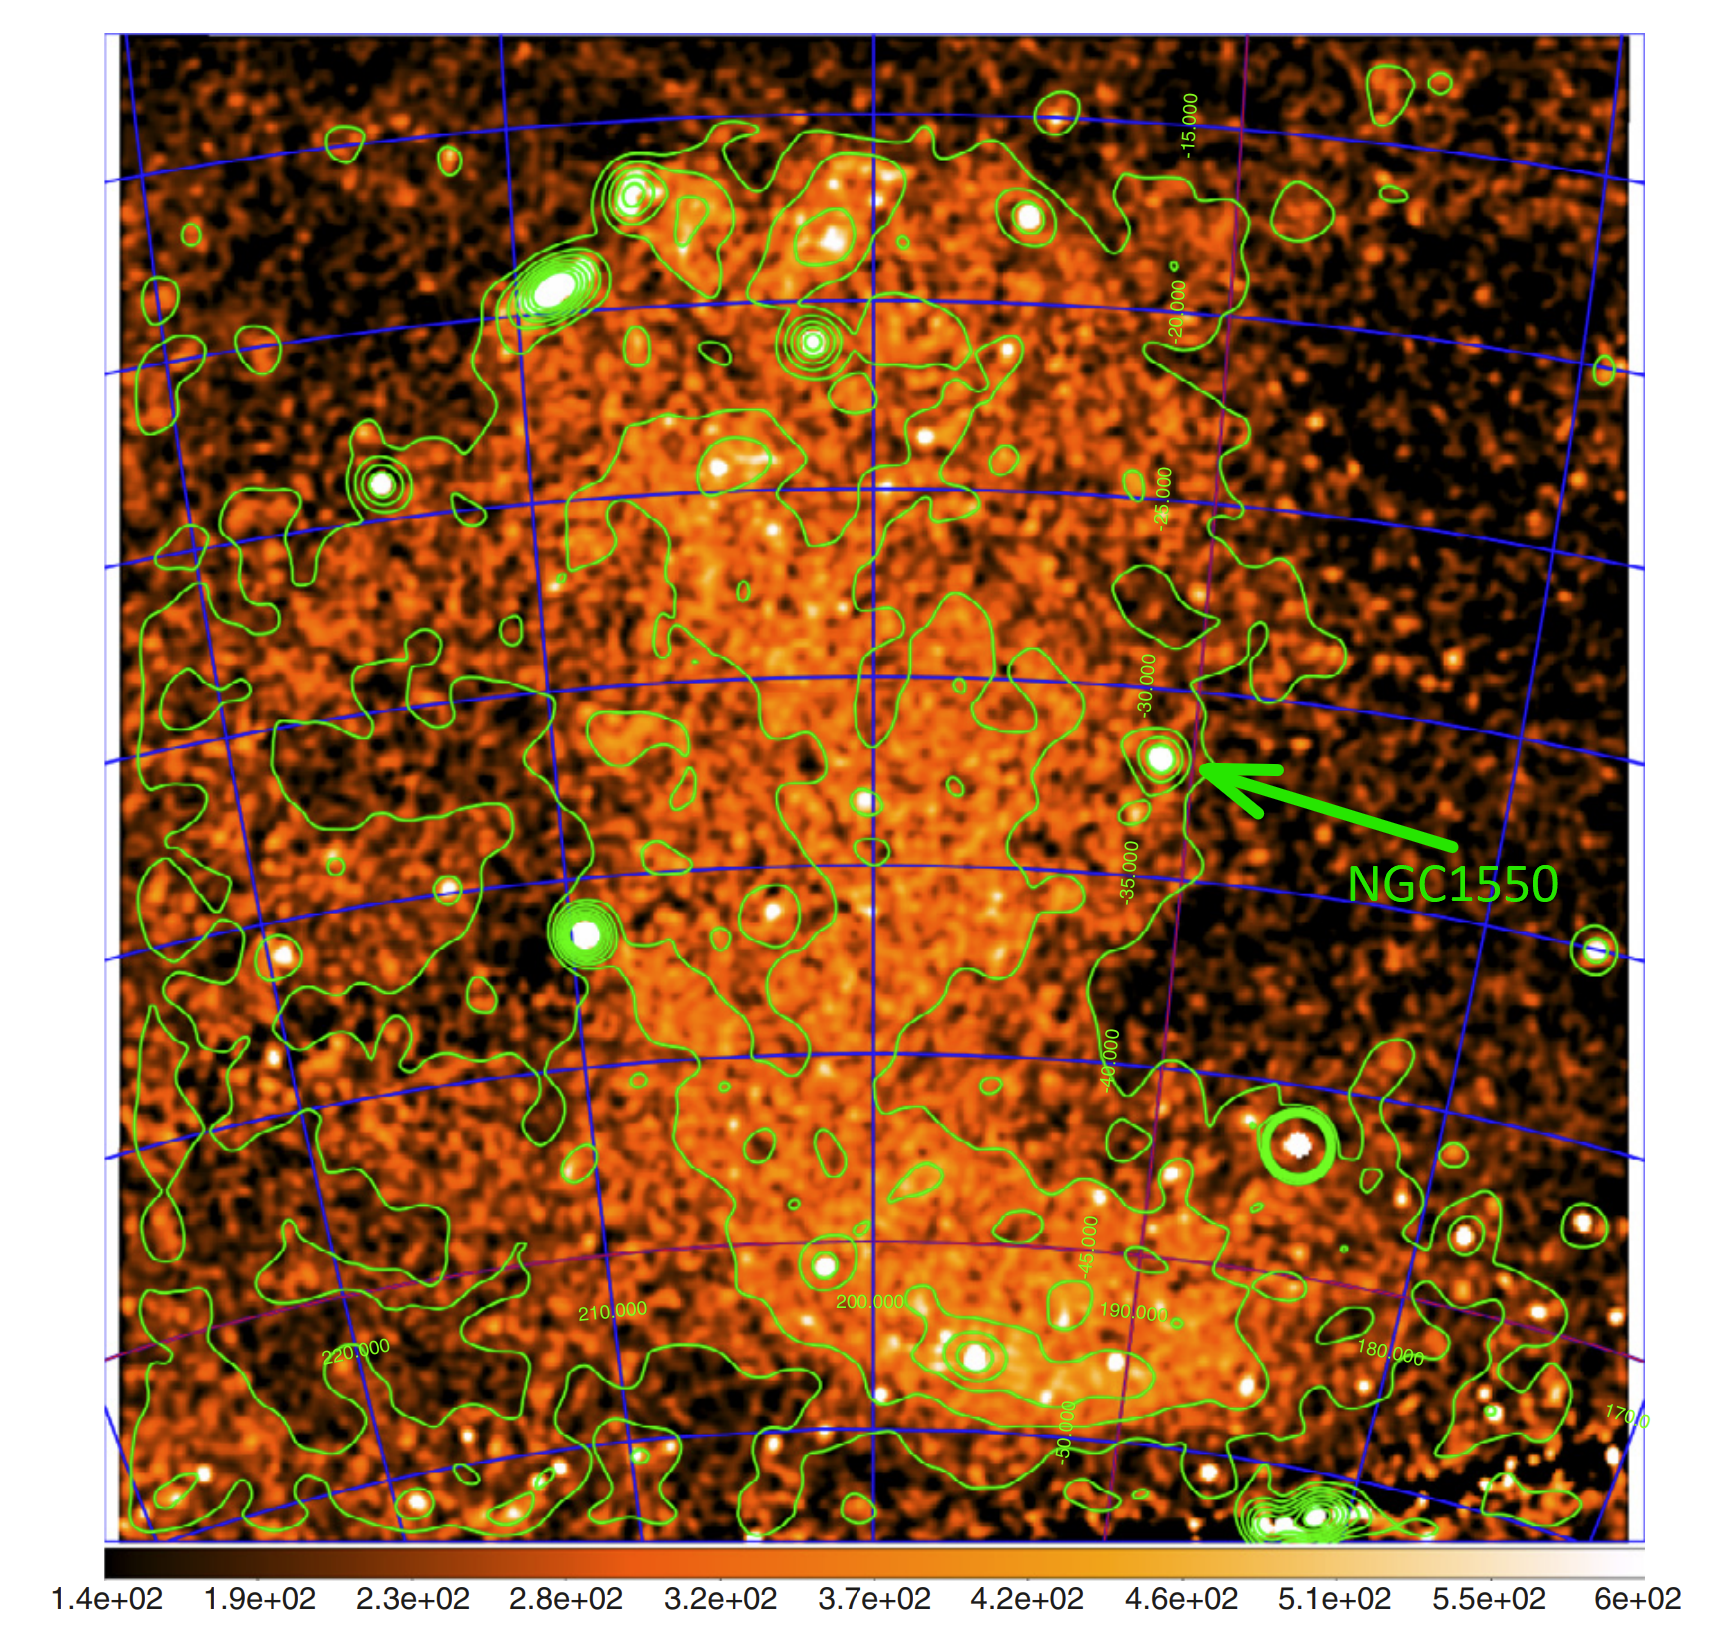
\includegraphics[width=0.7\textwidth]{data_reduction/rosat_orion_supper_bubble.png}
    \caption{X-ray map in galactic coordinates of the Orion-Eridanus superbubble in the \SIrange{0.5}{2.0}{\kilo\electronvolt} band from the ROSAT all-sky survey. The colorbar units are \(10^{-6}\,\text{cts}\cdot\text{arcmin}^{-2}\text{s}^{-1}\) and the contour levels are 220, 300, 380,
    460, 540, 620, 700. The image was taken from \cite{Krause_2014}. The green arrow and label were added to highlight the position of NGC1550.}
    \label{fig:orion_superbubble}
\end{figure}
\paragraph*{Non-X-ray Background (NXB):} The non-X-ray background consists of two main components: highly variable soft protons flares (SPF) from the solar corona and Earth's magnetosphere, which can be focused onto detectors, and energetic Galactic Cosmic Ray (GCR) primaries, which interact with the detector to produce secondary particles. While primary GCR events can mostly be discarded by onboard processing, the secondary particles deposit charge in the detector, making it challenging to distinguish them from true X-ray events. This is generally referred to as the particle-induced background (PIB) (\cite{Bulbul_2020}). 
\paragraph*{eROSITA light leak:} Shortly after the launch of eROSITA, it was observed that CCDs lacking an on-chip filter (TM9) recorded a notably higher number of events. This was attributed to optical and ultraviolet light from the Sun entering the CCD through an unidentified gap in the detector shielding, and was subsequently termed \enquote{light-leak} (\cite{Predehl2021}).
\paragraph*{\(N_\text{H}\) absorption:} 
As X-rays travel to the detector, they undergo photoelectric absorption in the interstellar and intergalactic medium. The cross-section \(\sigma \propto E^{-3}\) is inversely proportional to energy, causing a bias toward harder X-rays, as they interact less. Additionally, the cross-section is proportional to the atomic number, \(\sigma \propto Z^5\), making metal abundance crucial for energies \(\gtrsim \SI{0.2}{\kilo\electronvolt}\) (\cite{Willingale2013}).

